% Pitch deck - Stats (El Bloomberg de los datos publicos del Peru)
% Compilar: latexmk -pdf pitch_stats.tex   (o pdflatex dos veces)
\documentclass[aspectratio=169,11pt]{beamer}
\usepackage[utf8]{inputenc}
\usepackage[T1]{fontenc}
\usepackage{helvet}
\renewcommand{\familydefault}{\sfdefault}
\usepackage{graphicx}
\usepackage{booktabs}
\usepackage{array}

% --- Paleta de marca (del logo) ---
\definecolor{AzulStats}{RGB}{15,76,129}
\definecolor{AzulClaro}{RGB}{46,117,182}
\definecolor{NaranjaStats}{RGB}{238,125,34}
\definecolor{GrisTexto}{RGB}{55,60,68}
\definecolor{GrisSuave}{RGB}{120,128,138}

\setbeamertemplate{navigation symbols}{}
\setbeamercolor{normal text}{fg=GrisTexto}
\setbeamercolor{structure}{fg=AzulStats}
\setbeamercolor{frametitle}{fg=AzulStats}
\setbeamercolor{title}{fg=AzulStats}
\setbeamercolor{itemize item}{fg=NaranjaStats}
\setbeamercolor{itemize subitem}{fg=AzulClaro}
\setbeamercolor{block title}{fg=white,bg=AzulStats}
\setbeamercolor{block body}{bg=AzulStats!8,fg=GrisTexto}
\setbeamerfont{frametitle}{series=\bfseries,size=\Large}
\setbeamerfont{block title}{series=\bfseries}
\setbeamertemplate{itemize item}{\small\raise0.4pt\hbox{\textbullet}}
\setbeamertemplate{itemize subitem}{\scriptsize\raise0.4pt\hbox{\textbullet}}

% Titulo de frame con subrayado naranja
\setbeamertemplate{frametitle}{%
  \vspace*{0.45cm}\hspace*{0.5cm}%
  {\usebeamerfont{frametitle}\usebeamercolor[fg]{frametitle}\insertframetitle}\par
  \hspace*{0.5cm}{\color{NaranjaStats}\rule{2.1cm}{2.2pt}}%
  \vspace*{0.05cm}%
}

% Pie de pagina con marca
\setbeamertemplate{footline}{%
  \hbox{\begin{beamercolorbox}[wd=\paperwidth,ht=2.6ex,dp=1.3ex,leftskip=0.5cm,rightskip=0.5cm]{}%
    {\footnotesize\color{AzulStats}\textbf{Stats}\ \color{NaranjaStats}|\ \color{GrisSuave}El Bloomberg de los datos públicos del Perú}%
    \hfill {\footnotesize\color{GrisSuave}\insertframenumber\,/\,\inserttotalframenumber}%
  \end{beamercolorbox}}%
}

\newcommand{\impacto}[1]{{\Large\color{AzulStats}\textbf{#1}}}

\begin{document}

% ---------- Portada ----------
{\setbeamertemplate{footline}{}
\begin{frame}[plain]
  \centering
  \vspace{0.5cm}
  
\includegraphics[height=2.9cm]{Logo_Stats.png}\par
  \vspace{0.35cm}
  {\color{NaranjaStats}\rule{4.5cm}{2.2pt}}\par
  \vspace{0.5cm}
  {\Large\color{AzulStats}\textbf{El Bloomberg de los datos públicos del Perú}}\par
  \vspace{0.25cm}
  {\normalsize\color{GrisTexto}Recopilamos información pública y la volvemos utilizable:\\ en cualquier lugar, en cualquier momento.}\par
  \vspace{0.9cm}
  {\small\color{AzulStats}\textbf{Manuel Alfredo Arriola Montenegro}\ \ \color{GrisSuave}--- solo founder}\par
  \vspace{0.15cm}
  {\footnotesize\color{GrisSuave}Data Science con Python 2026-I\ \ $\cdot$\ \ Universidad del Pacífico\ \ $\cdot$\ \ Proyecto Final}\par
\end{frame}}

% ---------- One-liner ----------
\begin{frame}{¿Qué es Stats?}
  \vspace{0.3cm}
  \begin{center}
    \impacto{Somos el Bloomberg de los datos públicos del Perú.}
  \end{center}
  \vspace{0.5cm}
  Bloomberg tomó la data financiera, la volvió utilizable al instante y construyó un imperio por
  suscripción. \textbf{La data pública del Perú es igual de valiosa y está igual de desordenada.}\par
  \vspace{0.45cm}
  \begin{block}{}
    \textbf{Stats} recopila la data pública del Perú y la vuelve utilizable para tesistas e
    investigadores. Empezamos por la joya de la corona: la \textbf{ENAHO}.
  \end{block}
\end{frame}

% ---------- Founder ----------
\begin{frame}{Founder}
  \textbf{Manuel Alfredo Arriola Montenegro} --- economista (UP), solo founder.\par
  \vspace{0.5cm}
  \begin{itemize}
    \item \textbf{Founder--market fit:} sufro la ENAHO en carne propia, en tesis y econometría.
      Sé exactamente dónde duele.
    \item \textbf{Cubro los roles con IA:} \textcolor{AzulClaro}{Claude Code es mi CTO} --- construyó
      el backend de datos y la app en días; yo dirijo y reviso cada decisión.
    \item \textbf{Ejecución:} de cero a un MVP vivo, con repositorio profesional y CI, en menos de
      dos semanas.
  \end{itemize}
\end{frame}

% ---------- Problema ----------
\begin{frame}{El problema}
  La \textbf{ENAHO} es la principal fuente de pobreza, empleo e ingresos del Perú.\par
  \vspace{0.35cm}
  \begin{itemize}
    \item Pero llega en \textbf{decenas de módulos}, 3 metodologías, \textbf{+70 mil variables} y
      casi 30 años, con codificación incómoda.
    \item Encontrar una variable y bajar la base correcta toma \textbf{horas}. El portal de INEI a
      veces no responde.
    \item Lo sufren \textbf{tesistas, docentes-investigadores, analistas del sector público y
      consultoras}.
  \end{itemize}
  \vspace{0.3cm}
  \begin{block}{}
    Hoy lo resuelven a mano: Excel, descargas y prueba--error sobre el portal de INEI.
  \end{block}
\end{frame}

% ---------- Insight ----------
\begin{frame}{El insight}
  \vspace{0.4cm}
  \begin{center}
    \impacto{El valor no es la data. Es la capa que la ordena.}
  \end{center}
  \vspace{0.6cm}
  \begin{itemize}
    \item Bloomberg no vende los precios de las acciones (son públicos): vende el
      \textbf{acceso instantáneo} a ellos.
    \item Stats no vende la ENAHO (es pública): vende \textbf{encontrar la variable correcta en
      segundos} y ver el cuestionario en la \textbf{página exacta}.
  \end{itemize}
\end{frame}

% ---------- Solucion ----------
\begin{frame}{La solución}
  \begin{columns}[T]
    \begin{column}{0.56\textwidth}
      \small
      \begin{itemize}
        \item \textbf{Explorador} de módulos con sinopsis curada.
        \item \textbf{Diccionario} de +70 mil variables, buscable: en qué módulos y años aparece cada una.
        \item \textbf{Visor de cuestionario} (el diferenciador): la pregunta exacta del PDF, \textcolor{NaranjaStats}{resaltada}.
        \item \textbf{Indicadores} listos (pobreza, ingreso) por dominio y departamento, ponderados.
        \item \textbf{Descargas} listas para Stata, SPSS y Python.
      \end{itemize}
      \vspace{0.1cm}
      {\footnotesize\color{AzulStats}\textbf{Offline-first}: no depende de que INEI esté arriba.}
    \end{column}
    \begin{column}{0.44\textwidth}
      \centering
      \fbox{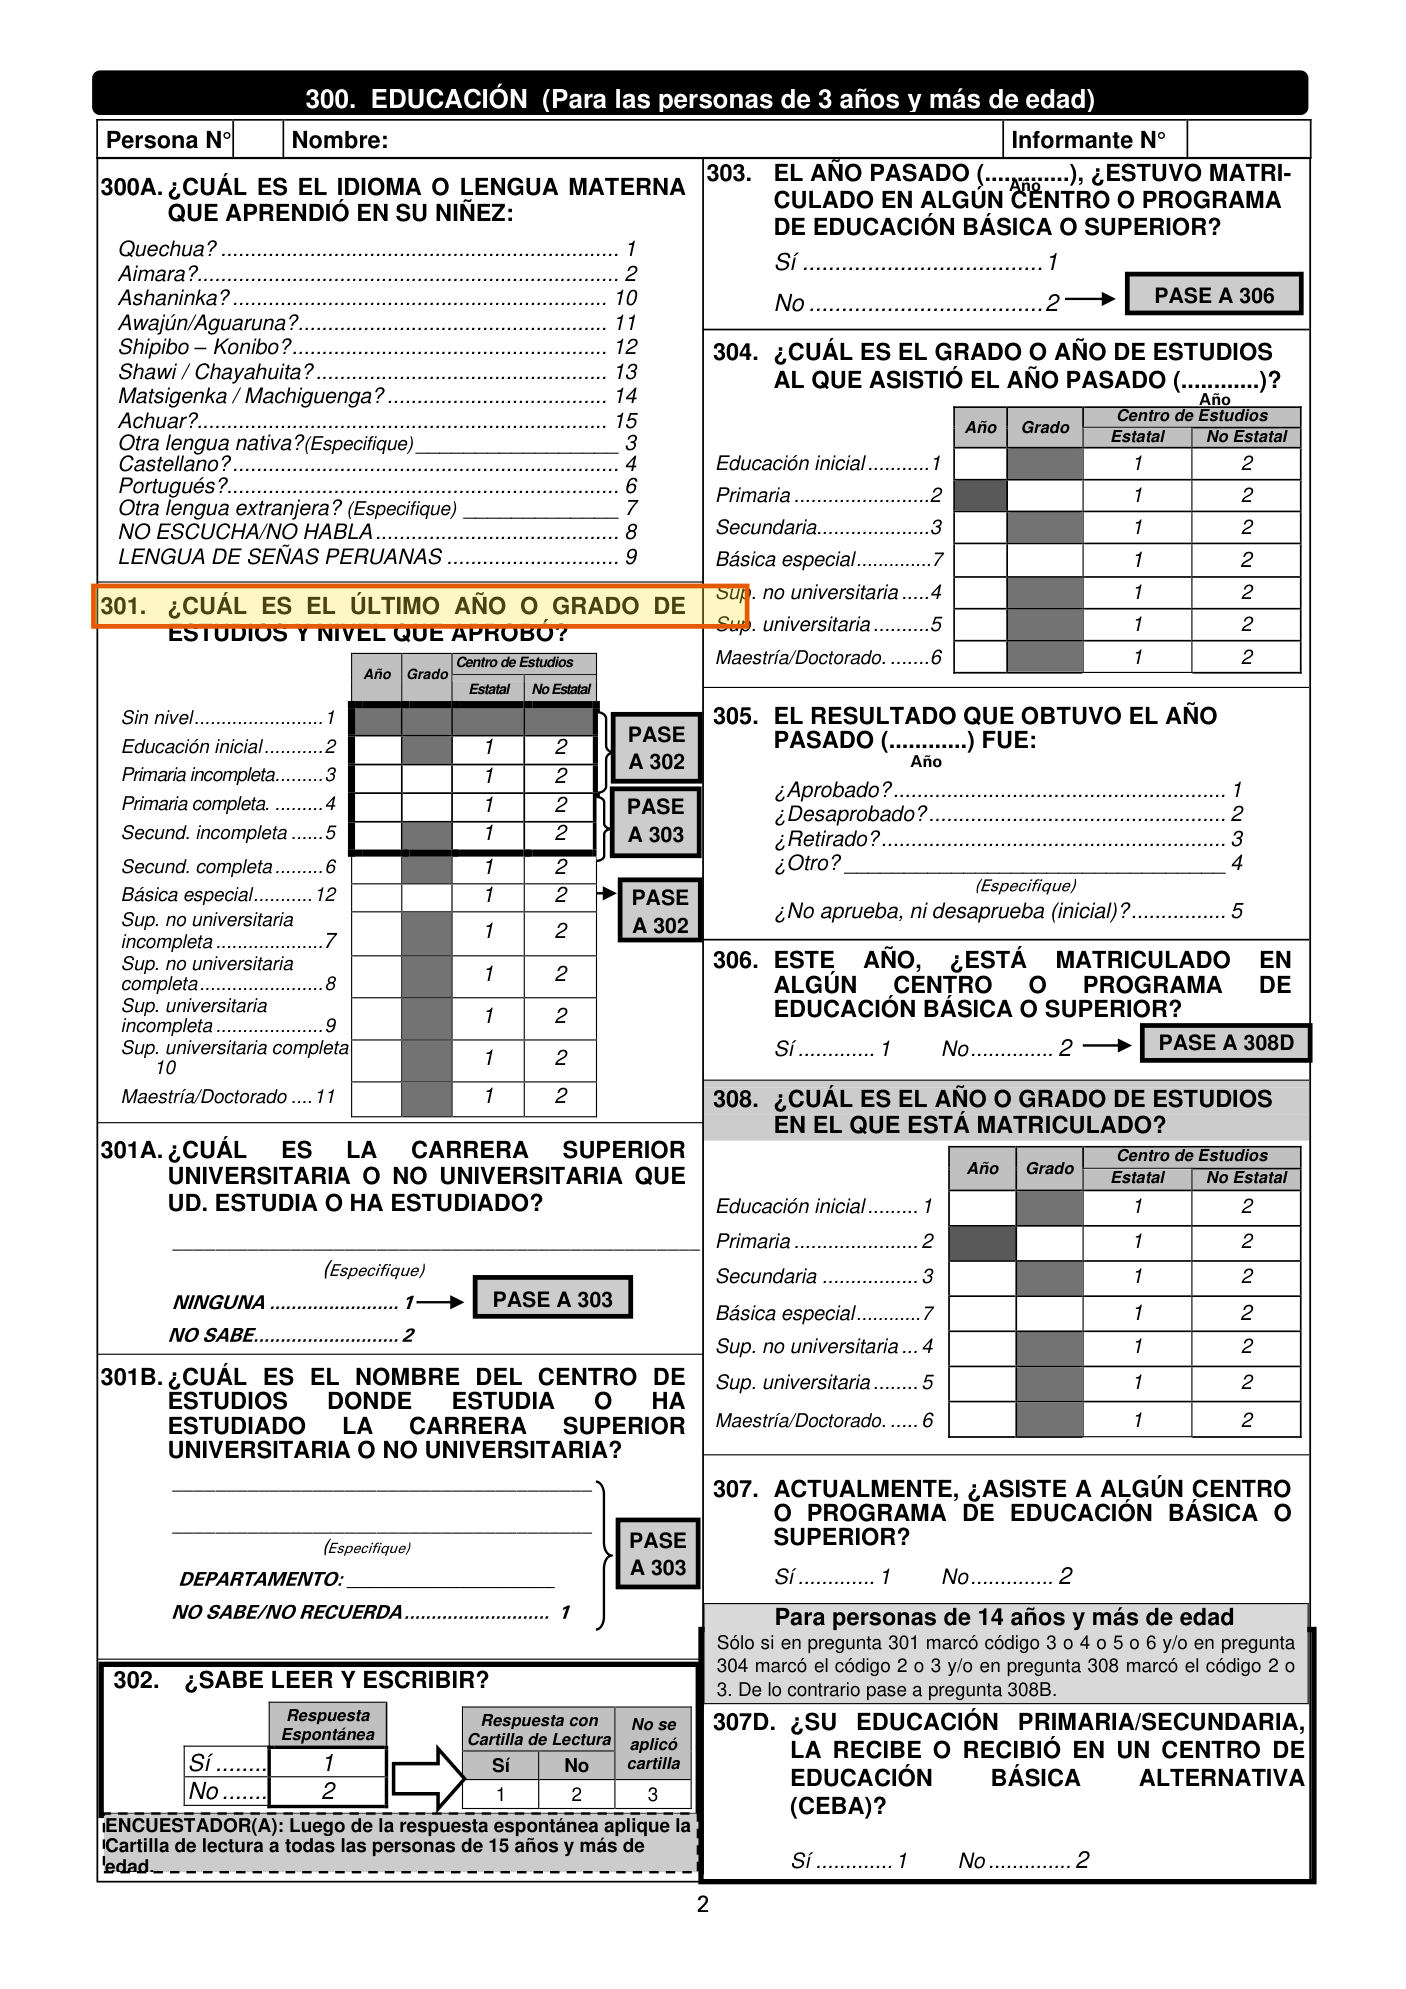
\includegraphics[width=\linewidth,height=5.8cm,keepaspectratio]{demo_cuestionario.png}}\\[2pt]
      {\scriptsize\color{GrisSuave}Variable \texttt{p301} $\to$ su pregunta resaltada.}
    \end{column}
  \end{columns}
\end{frame}

% ---------- Demo ----------
\begin{frame}{Demo en vivo}
  \begin{columns}[T]
    \begin{column}{0.5\textwidth}
      \vspace{0.5cm}
      \impacto{$\rightarrow$ Demostración en vivo}\par
      \vspace{0.4cm}
      Indicadores reales de la ENAHO 2024, ponderados con el factor de expansión, por
      \textbf{departamento}, descargables como imagen o Excel.\par
      \vspace{0.45cm}
      {\setlength{\fboxsep}{7pt}%
       \href{https://stats-demo.streamlit.app/}{\colorbox{NaranjaStats}{\color{white}\textbf{Abrir demo en vivo}}}}\par
      \vspace{0.25cm}
      {\small\href{https://stats-demo.streamlit.app/}{\textcolor{AzulClaro}{\texttt{stats-demo.streamlit.app}}}}\\[3pt]
      {\small\color{GrisSuave}Plan B: video de respaldo.}
    \end{column}
    \begin{column}{0.5\textwidth}
      \centering
      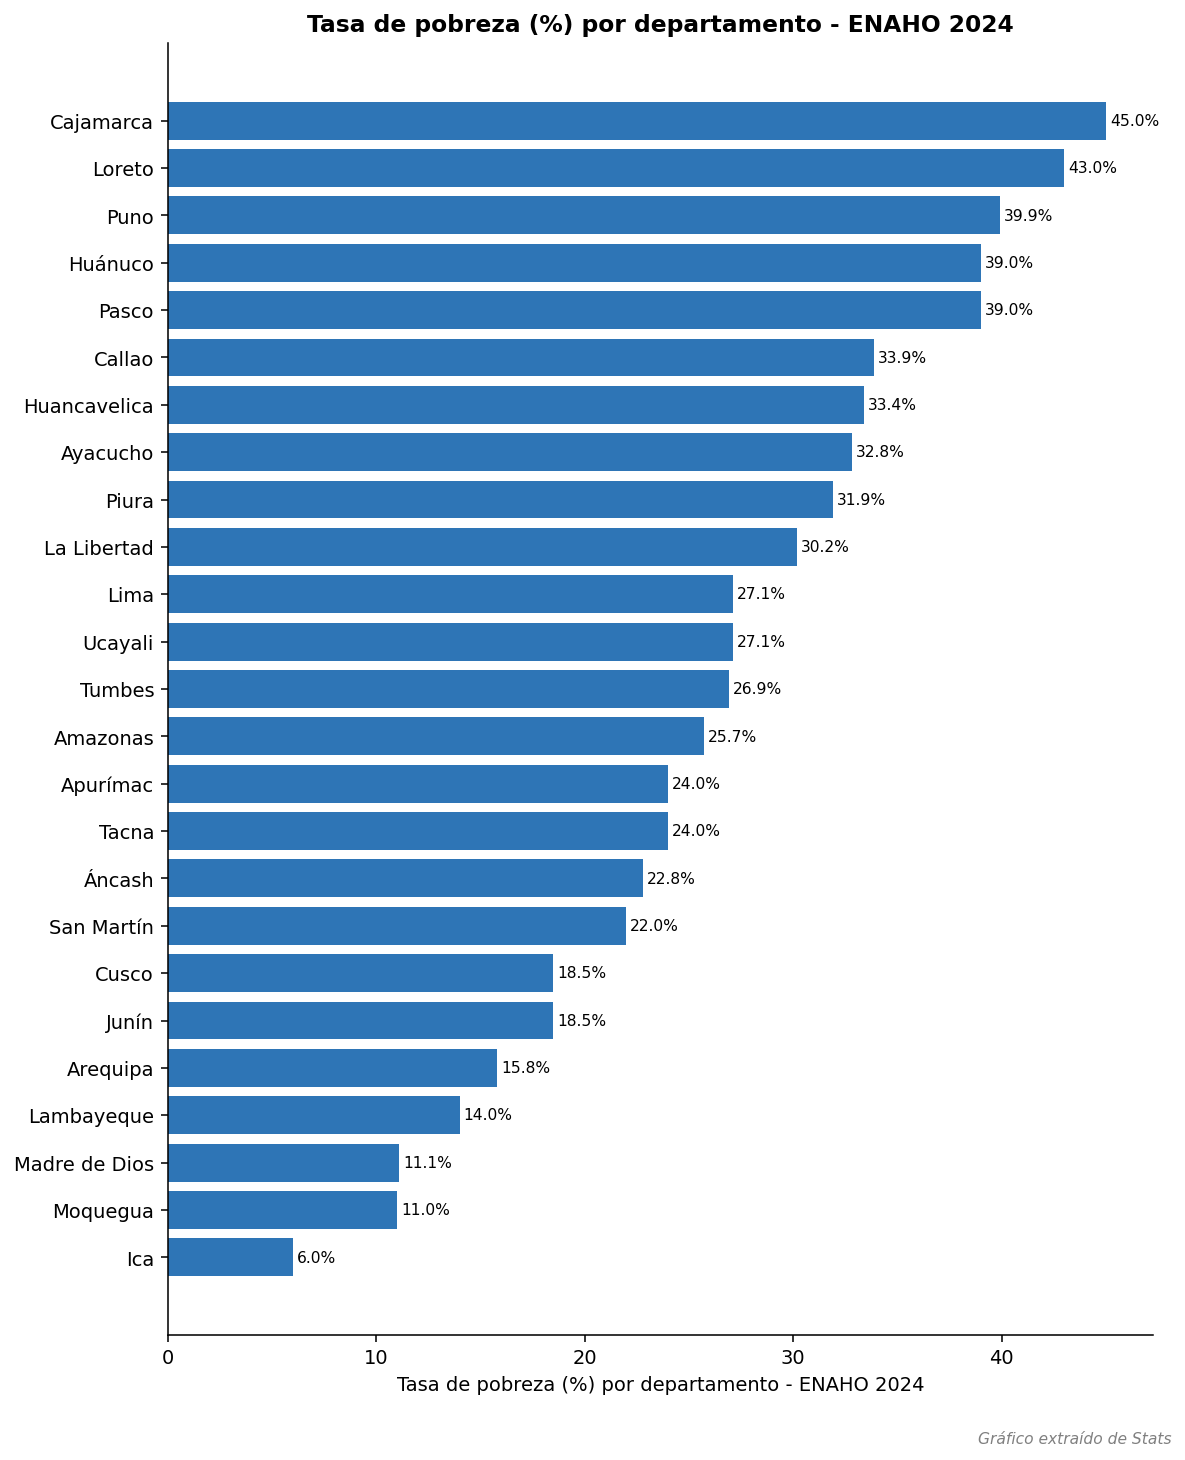
\includegraphics[width=\linewidth,height=6.2cm,keepaspectratio]{demo_pobreza.png}
    \end{column}
  \end{columns}
\end{frame}

% ---------- Arquitectura ----------
\begin{frame}{Arquitectura}
  \vspace{0.05cm}
  \begin{center}
    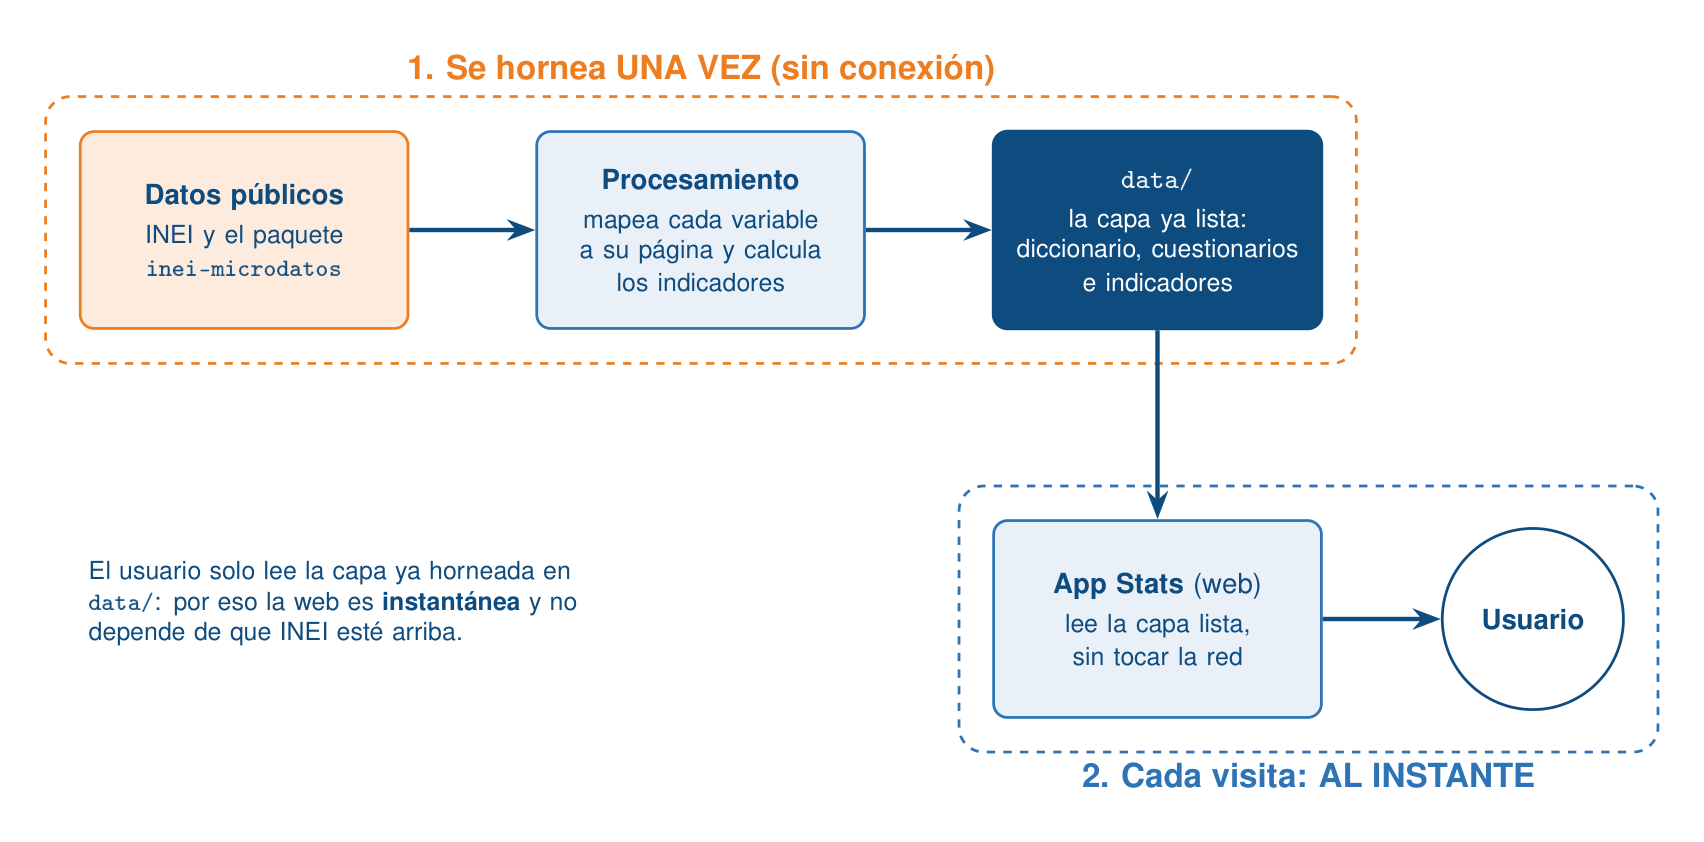
\includegraphics[width=0.97\linewidth,height=5.2cm,keepaspectratio]{arquitectura.png}
  \end{center}
  \vspace{0.1cm}
  {\footnotesize\color{GrisSuave}Publicado en Streamlit Cloud desde GitHub. Solo Descargas baja de INEI en vivo.}
\end{frame}

% ---------- Why now ----------
\begin{frame}{¿Por qué ahora?}
  \begin{itemize}
    \item \textbf{Agentes de código} (Claude Code): una sola persona construye el backend y la app
      en \textbf{días}, no en meses.
    \item \textbf{\texttt{inei-microdatos}}: catálogo e índice de +500 mil variables, offline.
    \item \textbf{Document AI / OCR} (pdfplumber + PaddleOCR): mapear cada variable a su
      \textbf{página exacta} del cuestionario.
  \end{itemize}
  \vspace{0.4cm}
  \begin{block}{}
    Hace 3 años esto era un equipo y varios meses. Hoy es un \textbf{solo founder} y una semana.
  \end{block}
\end{frame}

% ---------- Mercado ----------
\begin{frame}{Mercado: de lo amplio a lo alcanzable}
  \begin{center}
  \setlength{\fboxsep}{6pt}
  \colorbox{AzulStats}{\parbox{0.93\textwidth}{\centering\color{white}
    \textbf{Mercado total}\; (todos los que usan la ENAHO en el Perú)\\[1pt]
    \small 97 universidades licenciadas $\cdot$ $\sim$1,2 M de estudiantes $\cdot$ sector público y
    cooperación $\;\Rightarrow\;$ \textbf{50--80 mil usuarios}}}\\[5pt]
  \colorbox{AzulClaro}{\parbox{0.72\textwidth}{\centering\color{white}
    \textbf{A quienes podemos servir hoy}\\[1pt]
    \small Economía y ciencias sociales con tesis, más sector público y ONG
    $\;\Rightarrow\;$ \textbf{$\sim$5--10 mil usuarios}}}\\[5pt]
  \colorbox{NaranjaStats}{\parbox{0.66\textwidth}{\centering\color{white}
    \textbf{Meta realista a 12 meses}\\[1pt]
    \small \textbf{8--15 cuentas institucionales} $\cdot$ $\sim$500--1\,000 usuarios\\
    Cabeza de playa: UP, PUCP, ULIMA, UNMSM}}
  \end{center}
  \vspace{0.15cm}
  {\footnotesize\color{GrisSuave}TAM / SAM / SOM en jerga de negocios. \;Fuentes: SUNEDU (2023), RENACYT, INEI.}
\end{frame}

% ---------- Modelo de negocio ----------
\begin{frame}{Modelo de negocio}
  Suscripción, como Bloomberg: \textbf{B2B + freemium}.\par
  \vspace{0.25cm}
  \begin{center}\small
  \renewcommand{\arraystretch}{1.2}
  \begin{tabular}{>{\raggedright}p{3.2cm} l >{\raggedright\arraybackslash}p{6.4cm}}
    \toprule
    \textbf{\color{AzulStats}Plan} & \textbf{\color{AzulStats}Precio} & \textbf{\color{AzulStats}Para quién} \\
    \midrule
    Tesista (Free) & S/. 0 & Búsqueda, explorador, indicadores y visor. Gancho de adquisición. \\
    \textbf{Pro} & \textbf{S/. 39 / mes} & Descargas ilimitadas, exportar a PNG/Excel, multi-año. \\
    \textbf{Institucional} & \textbf{desde S/. 8\,000 / año} & Cuentas por facultad, asientos múltiples, soporte. \\
    \bottomrule
  \end{tabular}
  \end{center}
  \vspace{0.2cm}
  {\small{\color{AzulStats}\textbf{Contribution margin $>$ 90\%}}: data pública, metadata pre-horneada y hosting casi gratis.}
\end{frame}

% ---------- Competencia y moat ----------
\begin{frame}{Competencia y moat}
  \begin{center}\small
  \renewcommand{\arraystretch}{1.15}
  \begin{tabular}{>{\raggedright}p{5.0cm} >{\raggedright\arraybackslash}p{7.3cm}}
    \toprule
    \textbf{\color{AzulStats}Alternativa} & \textbf{\color{AzulStats}Limitación} \\
    \midrule
    Portal de microdatos de INEI & Gratis pero crudo: sin búsqueda de variables ni visor. \\
    Hacerlo a mano (Excel) & Horas por variable; propenso a errores (el \textit{status quo}). \\
    Paquetes / código (R, \texttt{inei-microdatos}) & Potentes, pero solo para programadores. \\
    Stata / SPSS & Herramientas de análisis, no de descubrimiento. \\
    \bottomrule
  \end{tabular}
  \end{center}
  \vspace{0.15cm}
  {\small\color{AzulStats}\textbf{Moat:} la capa curada y el \textbf{dataset propio variable $\to$ página
  del cuestionario} (difícil de replicar), más la marca y la comunidad.}
\end{frame}

% ---------- Go to market ----------
\begin{frame}{Go-to-market}
  \begin{itemize}
    \item \textbf{Primeros 10:} compañeros tesistas y profesores de la UP (founder--market fit), en
      talleres de tesis y cursos de econometría.
    \item \textbf{Primeros 100:} departamentos de economía y ciencias sociales de UP, PUCP, ULIMA y
      UNMSM; asesores de tesis; la red CIES; comunidades de datos en LinkedIn.
    \item \textbf{Primeros 1\,000:} las 97 universidades, unidades del sector público (MEF,
      ministerios, gobiernos regionales) y consultoras; alianzas con bibliotecas e INEI.
  \end{itemize}
\end{frame}

% ---------- Traccion y roadmap ----------
\begin{frame}{Tracción y roadmap}
  \textbf{Hoy:} MVP \textcolor{NaranjaStats}{\textbf{vivo}} con ENAHO 2024 --- cinco pestañas,
  indicadores reales y visor de cuestionario. Repositorio profesional con CI y commits repartidos.\par
  \vspace{0.45cm}
  \begin{itemize}
    \item \textbf{3 meses:} todos los años de la ENAHO + asistente con IA (API de Claude).
    \item \textbf{6 meses:} ENDES, CENAGRO, ENAPRES --- toda la microdata de INEI.
    \item \textbf{12 meses:} MEF, BCRP, censos. \textbf{Todo dato público del Perú en un solo lugar.}
  \end{itemize}
\end{frame}

% ---------- Vision LATAM ----------
\begin{frame}{Visión: de Perú a toda LATAM}
  El mismo problema existe en toda la región: cada país tiene su \textbf{encuesta nacional de
  hogares}, igual de fragmentada. El modelo de Stats se replica sin fricción.\par
  \vspace{0.35cm}
  \begin{columns}[T]
    \begin{column}{0.5\textwidth}
      \small
      \begin{itemize}
        \item \textbf{Perú} --- ENAHO \textcolor{NaranjaStats}{(hoy)}
        \item \textbf{Chile} --- CASEN
        \item \textbf{México} --- ENIGH
        \item \textbf{Colombia} --- GEIH
      \end{itemize}
    \end{column}
    \begin{column}{0.5\textwidth}
      \small
      \begin{itemize}
        \item \textbf{Argentina} --- EPH
        \item \textbf{Brasil} --- PNAD
        \item \textbf{Uruguay} --- ECH
        \item \textbf{Ecuador} --- ENEMDU
      \end{itemize}
    \end{column}
  \end{columns}
  \vspace{0.35cm}
  \begin{center}
    \impacto{Stats: el Bloomberg de los datos públicos de Latinoamérica.}
  \end{center}
\end{frame}

% ---------- The ask ----------
\begin{frame}{The ask}
  \vspace{0.2cm}
  \begin{block}{}
    Buscamos \textbf{S/. 50\,000 (pre-seed)} para 6 meses: integrar \textbf{5 encuestas más},
    lanzar el plan institucional y cerrar las \textbf{primeras 10 cuentas pagas}.
  \end{block}
  \vspace{0.4cm}
  \begin{center}
    
\includegraphics[height=1.55cm]{Logo_Stats.png}\par
    \vspace{0.25cm}
    {\large\color{AzulStats}\textbf{El Bloomberg de los datos públicos del Perú}}\par
    \vspace{0.12cm}
    {\small\color{GrisSuave}\textit{``Make something people want.''}\ ---\ Y Combinator}\par
    \vspace{0.12cm}
    {\footnotesize\color{AzulStats}ma.arriolam@alum.up.edu.pe}
  \end{center}
\end{frame}

\end{document}
